For the estimation of the rigid concepts the \acrfull{tps} mass and the structural mass estimate are combine to yield a single value. This estimation is based on reference mission. Steinfeldt \cite{Steinfeldt2009} provides one such mass estimate for high mass Mars entry concept. Two concept are considered a slender and a blunt body of which the latter is our primary interest. The reference missions used in this analysis are all of the blunt body type, similar to the rigid concept considered in this report. The estimation provided below are all meant for such a blunt body.

Some remarks must be made with regards to the use of these reference missions. Al tough rigid re-entry mission are plenty their relevance must be considered. Within this report a re-entry within the Martian atmosphere with a approach velocity of 7 [$km/s$]. Most relevant reference missions are either for a planet different from Mars. For the re-entry vehicles entering the Martian atmosphere the approach velocity may still be of a completely different order. Previously executed Martian entries were typically unmanned featuring Hohmann transfers to Mars. The mission at hand features however more direct transfer considering human constraints yielding different approach velocities. As such the estimation should incorporate in some extend the thermal and structural loading of the mission trajectory.

The estimation provided by Steinfeldt takes this into account, dividing the estimation into three different parts: The forebody thermal protection system mass, the forebody structural mass and the back shell structural and thermal protection system mass estimate. The estimation takes into account the size of the concept by using the vehicles total mass at the start of the re-entry (\gls{sym:m0}). The heat load is taken into account by using the heat load \gls{sym:Q} the structural loading is taken into account by using the peak dynamic pressure.

The mass estimate for the forebody thermal protection system is based in the heatload \gls{sym:Q} and is provided by \cite{Laub2004} in equation \ref{eq:tps_heat}:

\begin{equation}
\gls{sym:mheat} = (0.000091Q^{0.51575})\gls{sym:m0}
\label{eq:tps_heat}
\end{equation}

The mass estimate for the forebody  structure is conseqently given by equation \ref{eq:m_structure}:

\begin{equation}
\gls{sym:mstrcuture} = (0.0232 \gls{sym:q} ^{-0.1708} ) \gls{sym:m0}
\label{eq:m_structure}
\end{equation}

\begin{figure}[h]
	\centering
	\begin{subfigure}[b]{0.49\textwidth}
	\centering
	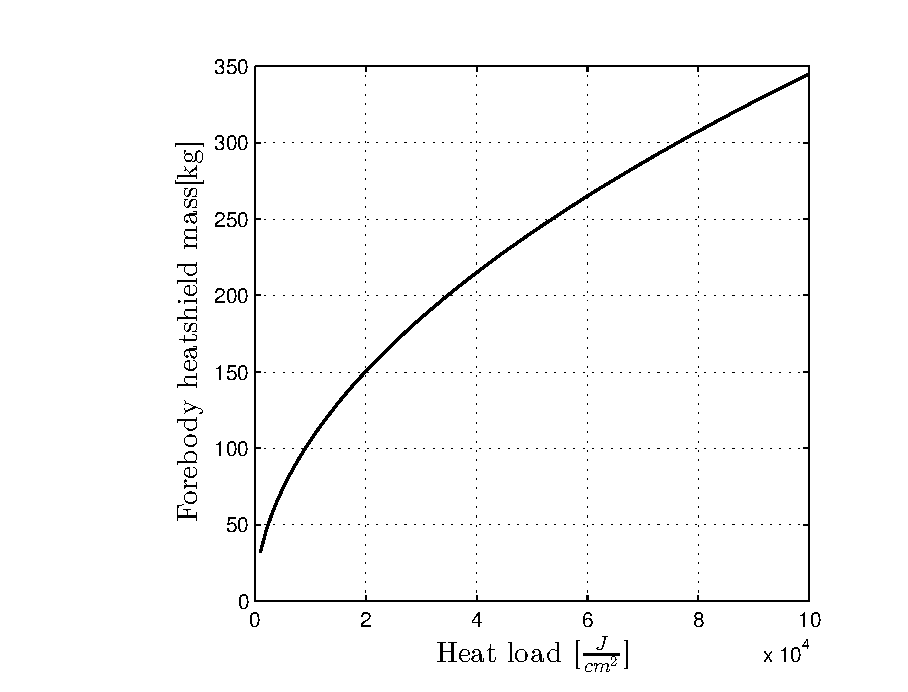
\includegraphics[width=1.0\textwidth]{Figure/rigidheat.eps}
	\caption{Empirical relation for the forebody heat shield mass} 
	\label{rigidheat}
	\end{subfigure}
	\begin{subfigure}[b]{0.49\textwidth}
	\centering
	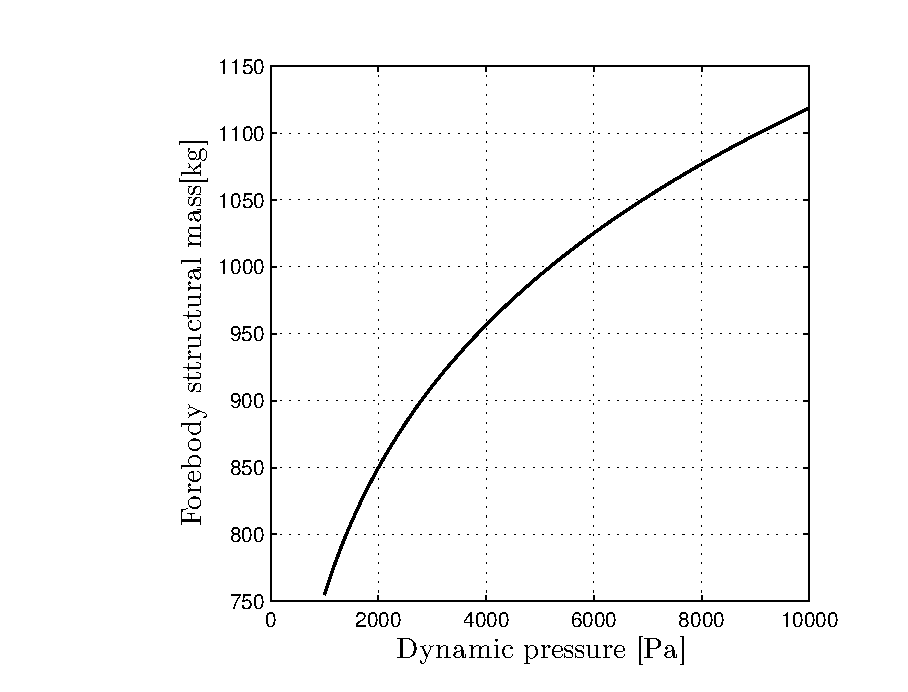
\includegraphics[width=1.0\textwidth]{Figure/rigidstruct.eps}
	\caption{Empirical relation for the forebody heat shield mass} 
	\label{fig:rigidstruct}
	\end{subfigure}
	\caption{Empirical relations for the forebody mass of a (blunt) rigid concept}
	\label{fig:rigid}
\end{figure}

Different from the inflatable concepts a rigid design features a additional back shell structure. 

m backshell 14 \%